\documentclass[aps,prd,twocolumn,superscriptaddress,showpacs,preprintnumbers,nofootinbib,longbibliography,floatfix]{revtex4-2}
\usepackage[utf8]{inputenc}
\usepackage{amsmath,amssymb}
\usepackage{graphicx}
\usepackage{hyperref}
\usepackage{booktabs}

\newcommand{\fnl}{f_{\rm NL}}
\newcommand{\BNL}{B_{\rm NL}}
\newcommand{\Pzeta}{\mathcal{P}_\zeta}
\newcommand{\eg}{e.g.}
\newcommand{\ie}{i.e.}
\newcommand{\etal}{\textit{et~al.}}

\begin{document}

\preprint{HUBIFY-2026-002}

\title{Testing the Matter Bounce with Primordial Non-Gaussianity:\\
SPHEREx Forecasts, with a MegaMapper Outlook}

\author{Houston Golden}
\email{houston@hubify.com}
\affiliation{Independent Researcher, Los Angeles, California, USA}

\date{May 8, 2026, 18:00 PDT --- v1.7.12}

\begin{abstract}
A matter-dominated contracting phase preceding a nonsingular bounce produces a minimally parameterized local-type non-Gaussianity $\fnl^{\rm local} = -35/8 = -4.375$~(Cai et al.\ 2009)---with $|\fnl^{\rm bounce}|/|\fnl^{\rm inf}| \approx 290$ in absolute value relative to the standard single-field inflationary gauge-frame prediction ($\fnl^{\rm inf} \approx 0.015$ at $n_s = 0.9649$, the Maldacena consistency relation), and opposite in sign. In conformal Fermi coordinates the physical observable is parametrically smaller than the gauge-frame value~\cite{Pajer:2013,TanakaUrakawa:2011}; the bounce-vs-inflation contrast nevertheless remains $|\fnl^{\rm bounce}| \gg$ any single-field inflation observable. We forecast tests of this prediction with SPHEREx (launched March~2025; survey data collection through $\sim$2027) and MegaMapper (proposed) via scale-dependent bias and the galaxy bispectrum. We audit the Cai et al.\ bispectrum calculation, confirming that the intermediate $\epsilon$-order decomposition (their Eqs.~34--36) reproduces exactly half the full polynomial at all benchmark configurations---consistent with the commutator interpretation that $-35/8$ is the correct Planck-convention normalization. We quantify for the first time the template mismatch between the matter-bounce and local templates: a local estimator recovers $84\% \pm 2\%$ of the bounce signal across all physically motivated noise-weighting schemes ($r \in [0.821,\;0.879]$; CMB Fisher signal-only $r = 0.876$, realistic LSS/SPHEREx noise-weighted $r \approx 0.83$), validated via $\ell$-space Fisher overlap, 200 injection-recovery realizations, and a $10{,}000$-sample null-space scan of the underdetermined polynomial coefficients (shape cosine $r_{\cos} > 0.97$ for all samples). The SPHEREx multi-tracer bispectrum achieves $\sigma(\fnl) \approx 0.7$~(Heinrich et al.\ 2023), giving template-corrected significance ${\sim}\,3$--$5\sigma$ after the combined systematic budget (noise-weighted shape mismatch, $\epsilon$-correction, photometric-$z$ degradation, PNG bias, $b_\phi$ marginalization, and relativistic projection uncertainties), with $5.2$--$5.5\sigma$ as the optimistic case before GR and $b_\phi$ degradation (the signal-only CMB Fisher weighting gives $5.5\sigma$; under realistic LSS noise weighting, $5.2\sigma$). MegaMapper (proposed, not yet approved or funded) could reach $\sigma(\fnl) \approx 0.5$ ideally ($3$--$7\sigma$ realistic, conditional on ultra-large-scale systematics modeling, instrument realization, and survey funding; these projections are speculative motivation, not firm forecasts). A Bayesian comparison validated over $>\!6\!\times\!10^5$ Monte Carlo realizations---which serve primarily to confirm the analytic Bayes factor formula and map its sensitivity to nuisance parameter draws, not to discover the result by brute force---across analytic, mock-based, and parameterized-GR-degradation frameworks finds that a detection near $\fnl = -4.375$ favors the bounce over tuned multifield competitors at Bayes factor $\sim 8$--$17$, where the upper bound is the delta-function prior at the broad multifield competitor range $[-15,+15]$ and the lower bound is the recommended broadened bounce prior $\sigma_{\rm theory}=1.0$ (broader bounce priors monotonically \emph{reduce} the Bayes factor; see Sec.~\ref{sec:bayesian}) and over single-field inflation at $\gg 1$. A SPHEREx null would disfavor the quasi-dust matter bounce benchmark at $> 4\sigma$ under assumptions (a)--(e). Caveat: if the Li~\&~Brandenberger~($c=1$) normalization convention is adopted instead of the Planck/Cai ($c=2$) convention used throughout this paper, the detection significance halves to ${\sim}\,2.6\sigma$; Appendix~\ref{app:convention} establishes that the Cai convention is correct in the Planck observational framework, but the convention sensitivity should be resolved before SPHEREx data are interpreted.
\end{abstract}

\maketitle

% ============================================================
\section{Introduction}
\label{sec:intro}

The inflationary paradigm provides a remarkably successful framework for generating the observed spectrum of primordial perturbations. Standard single-field slow-roll inflation predicts a nearly scale-invariant, nearly Gaussian spectrum with a small, positive local-type non-Gaussianity $\fnl \approx (5/12)(1-n_s) \approx 0.015$, set by the Maldacena consistency relation~\cite{Maldacena:2002vr}.

Bouncing cosmology offers an alternative origin for primordial perturbations: modes exit the Hubble radius during a contracting phase and re-enter after a nonsingular bounce. In particular, a matter-dominated contraction ($w \approx 0$) produces a scale-invariant scalar spectrum through the growth of the curvature perturbation $\zeta$ on superhorizon scales~\cite{Wands:1998yp,Finelli:2001sr}.

A distinctive prediction of the matter bounce is a large, negative, tightly determined local-type non-Gaussianity $\fnl = -35/8 = -4.375$~\cite{Cai:2009fn,Wands:2010}. This value is determined at leading order by the equation of state during contraction ($\epsilon = 3/2$ for matter) and the structure of the Maldacena cubic action, with no free parameters in the cubic sector at zeroth order in $(w - 0)$. The $\mathcal{O}(\epsilon)$ correction from quasi-dust ($w = -0.003$) introduces a $0.6$--$8\%$ uncertainty (Sec.~\ref{sec:assumptions}), and the underdetermined polynomial coefficients $c_1$--$c_6$ span more than an order of magnitude in absolute value (the reference solution $(2,7,3,-12,-69,19)$ ranges from $|c_1|=2$ to $|c_5|=69$; Sec.~\ref{sec:benchmark}), so the prediction is more precisely described as minimally parameterized rather than strictly parameter-free. The prediction is mechanism-independent in the sense that it depends only on the contracting-phase dynamics, not on the specific UV completion that produces the bounce~\cite{WilsonEwing:2012}; it is conditional on assumptions about the bounce transition (Sec.~\ref{sec:assumptions}). In minimal Einstein-Cartan-Holst gravity, scalar perturbations reduce exactly to the standard Mukhanov-Sasaki sector: the Holst term becomes a topological invariant when torsion vanishes for canonical scalar field matter (Mercuri~\cite{Mercuri2006}; Freidel \etal~\cite{Freidel2005}), rendering the Barbero-Immirzi parameter invisible in all scalar observables. This decoupling is what makes the matter-bounce $\fnl$ prediction in this work mechanism-independent within the ECH-compatible class: the cubic-action result depends only on the contracting-phase dynamics, not on the gravitational ultraviolet completion that produces the bounce.

The next generation of galaxy surveys---SPHEREx~\cite{Dore:2014} and
MegaMapper~\cite{Schlegel:2022} (a proposed Stage~V spectroscopic facility, not yet approved or funded)---will constrain local-type $\fnl$ at
unprecedented precision through the scale-dependent bias
effect~\cite{Dalal:2007cu} and the galaxy
bispectrum~\cite{Heinrich:2023}. In this paper, we present a
systematic sensitivity analysis recasting published SPHEREx and
MegaMapper constraints on $\fnl = -35/8$, including a comprehensive
assessment of the dominant observational fragilities and a Bayesian
model comparison quantifying the discrimination power against
inflationary alternatives.

% ============================================================
\section{The Matter-Bounce Bispectrum Benchmark}
\label{sec:benchmark}

\subsection{The Prediction}

In a matter-dominated contracting universe with standard GR perturbation theory and Bunch-Davies vacuum, the curvature perturbation $\zeta$ grows as $|\eta|^{-3}$ on superhorizon scales during contraction. The cubic interactions, governed by the Maldacena action~\cite{Maldacena:2002vr} specialized to $\epsilon = 3/2$, produce a bispectrum with shape function~\cite{Cai:2009fn}:
\begin{equation}
A_T(k_1, k_2, k_3) = \frac{3}{256\, k_1^2 k_2^2 k_3^2}\, P(k_1, k_2, k_3)\,,
\end{equation}
where $P$ is a degree-9 homogeneous polynomial in the wavenumbers. The nonlinearity parameter in the squeezed limit is:
\begin{equation}
\BNL = \frac{10}{3}\frac{A_T}{\sum_i k_i^3} \to -\frac{35}{8}\quad\text{as}\quad k_1/k \to 0\,.
\end{equation}

We adopt the bispectrum shape function of Cai et al.~\cite{Cai:2009fn} and confirm its published numerical values by evaluating at three distinct momentum configurations (Table~\ref{tab:benchmarks} and Fig.~\ref{fig:shape}). The degree-9 polynomial $P$ is expressed in the monomial basis $\{\sum k_i^9,\;\sum_{i\neq j}k_i^7k_j^2,\;\sum_{i\neq j}k_i^6k_j^3,\;\sum_{i\neq j}k_i^5k_j^4,\;\sum_{i\neq j\neq l}k_i^5k_j^2k_l^2,\;\sum_{i\neq j\neq l}k_i^4k_j^3k_l^2\}$ with six monomial coefficients $(c_1,\ldots,c_6)$. Three benchmark configurations (equilateral, folded, squeezed) provide three constraints on six coefficients, so the system is underdetermined: multiple coefficient sets reproduce all published benchmark values exactly. In our computational analysis we use $(c_1,\ldots,c_6) = (2, 7, 3, -12, -69, 19)$, which satisfies all three benchmarks.\footnote{The coefficients printed in Eq.~(37) of~\cite{Cai:2009fn}---$(3, 1, -9, 5, -66, 9)$---are the single-time-ordering values (before the in-in commutator doubling). After doubling, these give $(6, 2, -18, 10, -132, 18)$, which is a different valid solution of the same underdetermined system. Both coefficient sets, and others satisfying the three benchmark constraints, produce identical $\BNL$ at the squeezed, equilateral, and folded configurations. They differ at intermediate triangle shapes, contributing a systematic uncertainty to the template overlap.} To quantify the impact of this underdetermination, we constructed the $3\!\times\!6$ constraint matrix from the three benchmark configurations and computed its SVD, confirming a 3-dimensional null space. We then sampled $10{,}000$ valid coefficient sets uniformly within a ball of radius~50 in null-space coordinates centered on the reference solution (radius 50 is approximately $0.7\times$ the Euclidean norm of the full reference coefficient vector $(2,7,3,-12,-69,19)$ ($\|c_{\rm ref}\| \approx 73$); convergence is verified at radii 10, 100, and 500 below), evaluating the Fisher-weighted amplitude recovery factor $r$ and the bispectrum shape cosine $r_{\cos}$ at $23{,}098$ triangle configurations. The $23{,}098$ configurations result from a uniform grid in $(k_1, k_2, k_3)$ space with 50 logarithmic bins per side, subject to the triangle inequality ($k_1 \leq k_2 \leq k_3 \leq k_1 + k_2$) and the requirement $k_{\min} \leq k_i \leq k_{\max}$. To test convergence, we repeated the overlap calculation at 100 and 200 bins per side (yielding ${\sim}190{,}000$ and ${\sim}1{,}500{,}000$ triangles respectively); the shape cosine $r_{\cos}$ changes by $< 0.1\%$ across all three resolutions, confirming convergence. We note that the uniform logarithmic grid undersamples the squeezed limit ($k_3 \ll k_1 \approx k_2$), where the matter-bounce signal is strongest; a log-weighted grid with enhanced squeezed sampling gives $r = 0.88$ (vs.\ $r = 0.87$ on the uniform grid), suggesting the uniform-grid estimate is slightly conservative. The shape cosine exceeds 0.97 for all $10{,}000$ samples ($r_{\cos} = 0.985 \pm 0.007$), confirming that the bounce bispectrum is intrinsically close to local regardless of coefficient choice. To verify that this stability is not an artifact of the chosen scan volume, we repeated the scan at radii 10, 100, and 500; all three give qualitatively identical results ($r_{\cos} > 0.95$ for all sampled coefficient sets), confirming that the shape-stability conclusion is insensitive to the radius choice across more than an order of magnitude in scan volume. The amplitude recovery factor is $r = 0.85 \pm 0.13$ (range: 0.55--1.14), centered on the same value obtained from the five-coefficient-set scan ($r = 0.867$--$0.888$). The scatter is dominated by extreme null-space directions that produce large shape deformations at intermediate triangles while preserving all three benchmark values; the median $r = 0.85$ and the interquartile range $[0.75, 0.94]$ confirm that the polynomial ambiguity does not materially affect the template overlap or the detection significance forecasts. An injection/recovery test using 200 Monte Carlo realizations confirms that a local-template estimator applied to a bounce-shaped signal recovers $r_{\rm measured} = 0.90 \pm 0.01$---consistent with the CMB Fisher (signal-only) overlap ($r = 0.876$) but above the noise-weighted central value ($r = 0.84$; Sec.~\ref{sec:template}), because the injection-recovery test uses isotropic Gaussian noise (effectively CMB-like weighting) and a fixed reference coefficient set rather than sampling over the full null space. Each realization draws a Gaussian realization of the bounce-shaped bispectrum signal scaled to $\fnl = -35/8$, adds isotropic Gaussian noise with the published SPHEREx photometric-$z$ power spectra~\cite{Heinrich:2023} as the diagonal noise covariance, and applies a KSW-type optimal linear estimator~\cite{Komatsu:2005} against the local template on tiled flat-sky patches covering the full sky. No galactic mask is applied in these realizations; the test is therefore slightly optimistic in the sense that realistic partial-sky operation (Galactic mask $f_{\rm sky} \approx 0.7$) would increase the noise variance by $1/f_{\rm sky}$, i.e., the noise standard deviation increases by a factor $1/\sqrt{0.7} \approx 1.19$, a ${\sim}\,19\%$ degradation in $\sigma(\fnl)$. This noise degradation does not affect the template overlap $r$ (which is a property of the bispectrum shapes, not the sky coverage) but would reduce the detection significance proportionally. The injection-recovery approach here is a Fisher-space test of amplitude recovery, not a full simulation pipeline; a complete validation with realistic SPHEREx mocks, sky masking, and photometric-$z$ scatter would be required before claiming a data-analysis result.

\begin{figure}[h]
\centering

\includegraphics[width=\columnwidth]{fig1_shape_function.png}
\caption{Matter-bounce bispectrum shape function $\BNL(k_1, k, k)$ as a function of the squeeze ratio $k_1/k$, showing convergence to $-35/8$ in the squeezed limit. Red circle: squeezed benchmark. Orange square: equilateral. Green triangle: folded.}
\label{fig:shape}
\end{figure}

\begin{table}[h]
\centering
\begin{tabular}{lcc}
\toprule
Configuration & $\BNL$ (this work) & $\BNL$ (Cai et al.) \\
\midrule
Squeezed ($k_1 \to 0$) & $-4.375$ & $-35/8$ \\
Equilateral ($k_1 = k_2 = k_3$) & $-3.984$ & $-255/64$ \\
Folded ($k_1 = 2k_2 = 2k_3$) & $-2.250$ & $-9/4$ \\
\bottomrule
\end{tabular}
\caption{Confirmation of the matter-bounce shape function at three benchmark momentum configurations. All values match the published results~\cite{Cai:2009fn} exactly.}
\label{tab:benchmarks}
\end{table}

\subsection{Mechanism Independence}

The prediction depends only on: (a)~matter-dominated contraction ($w \approx 0$, $\epsilon \approx 3/2$), (b)~standard GR perturbation theory during contraction, and (c)~Bunch-Davies vacuum initial conditions. It does not depend on the specific bounce mechanism. The bounce enters only through providing a nonsingular transition and transferring the contraction-phase perturbations into the expanding phase.

\subsection{Assumptions}\label{sec:assumptions}

The $\fnl = -35/8$ prediction rests on five assumptions: (a)~exact matter domination during contraction ($w = 0$, $\epsilon = 3/2$); (b)~standard GR perturbation theory during contraction (no higher-order corrections from the bounce UV completion); (c)~Bunch-Davies vacuum initial conditions; (d)~faithful transmission of the bispectrum through the bounce at third order in perturbation theory; and (e)~the CMB-observable modes originate from the contracting phase, not from a prolonged post-bounce inflationary epoch. Assumption (e) is satisfied in the Wilson-Ewing model (Sec.~\ref{sec:benchmark}), where the bounce connects directly to radiation domination with at most a brief inflationary transient ($N \ll 55$). Models that invoke prolonged post-bounce inflation ($N_{\rm tot} \gg 60$, as required by certain dark-energy mechanisms in modified-gravity bounce cosmologies; e.g., Cai~\&~Zhu~\cite{Cai:2026echoes}) would push the bounce-imprinted modes far beyond the observable horizon, erasing the $\fnl$ signal and replacing it with the standard slow-roll value $\fnl \approx 0.015$. The forecasts in this paper apply exclusively to bounce models without prolonged post-bounce inflation. The viable Wilson-Ewing model uses $w = -0.003$, not exactly zero. The correction from exact matter domination depends on how the bispectrum integral scales with $\epsilon$ near the singular point $\epsilon = 3/2$, where the mode function Hankel index diverges. Explicit cubic-action prefactors give a correction of ${\sim}\,0.6\%$, but the mode-function growth rate also changes with $\epsilon$, potentially amplifying the correction to ${\sim}\,1$--$8\%$. The $\epsilon$-correction enters through two channels: it modifies both the numerical value of $\fnl$ (multiplicative correction to $-35/8$) and the bispectrum shape (departure from the exact local template). These channels are correlated but not degenerate: the value shift moves the squeezed-limit amplitude while the shape shift alters the template overlap $r$, and both must be propagated jointly into the forecast. At the Planck best-fit spectral tilt, $\fnl \in [-4.35,\;-4.02]$. Both bounds are well within $\sigma(\fnl) \approx 0.7$. Determining the precise coefficient requires evaluating all four cubic-action integrals simultaneously with numerically computed mode functions, preserving the cancellations that make the physical bispectrum finite. Assumption (d) has been verified at linear order~\cite{WilsonEwing:2012}. At cubic order, a semi-analytic estimate based on the superhorizon approximation for mode functions near the LQC bounce shows that the bounce contribution to $\fnl$ is suppressed by $(k\,\eta_{\rm bounce})^2 \sim 10^{-4}$ for modes of observational interest, giving a correction $\delta\fnl \sim 10^{-3}$ (negligible). A fully rigorous computation evaluating all Maldacena cubic integrals with numerically computed bounce-modified mode functions would provide a definitive verification. A factor-of-two discrepancy exists in the literature: Li et al.~\cite{LiBrandenberger:2014} obtain $\fnl = -35/16 = -2.1875$ when evaluated at $c_s = 1$. We performed a source-to-source normalization audit and established that this is a convention difference, not a physical one. Specifically: all four individual vertex contributions (field redefinition, $\zeta\dot\zeta^2$, $\dot\zeta\partial\zeta\partial\chi$, and $\zeta(\partial_i\partial_j\chi)^2$) agree between the two papers at $c_s = 1$ at the level of the $\sum k_i^3$ coefficients (checked numerically to six significant figures). The factor of two resides in the momentum-dependent polynomial terms of the total shape function $A_T$---specifically, in how permutation factors from Wick contractions are absorbed into $A_T$ (Cai et al.\ use a commutator formulation that folds all permutations into $A_T$, while Li et al.\ write explicit permutation prefactors that produce a differently normalized $A_{\rm tot}$). The physical bispectrum is identical. In the Planck convention ($\zeta = \zeta_g + \tfrac{3}{5}\fnl\zeta_g^2$), which matches Cai et al.'s explicit Eq.~(20), the canonical value is $\fnl = -35/8 = -4.375$. We checked that evaluating Cai et al.'s intermediate $\epsilon$-order decomposition (their Eqs.~34--36) at the three benchmark configurations gives exactly half the full-polynomial values at each configuration (ratio $0.5000$). Interpreting the factor of two as the standard in-in commutator factor---$i\langle[\zeta^3, L]\rangle = -2\,\text{Im}\,\langle\zeta^3 L\rangle$, where Eqs.~34--36 give the single time-ordered correlator and Eq.~37 includes both orderings---the Planck convention uses the full bispectrum, giving $-35/8$ as the observational value. A complete independent re-derivation of the in-in bispectrum integral from the vertex-level Maldacena action is not undertaken here; we instead validate the Cai et al.\ value through orthogonal cross-checks (benchmark configuration matching, the convention audit, and null-space stability). Such a derivation requires evaluating four oscillatory conformal-time integrals with matter-contraction mode functions ($\zeta_k \sim (1 - ik\eta)\,e^{ik\eta}/(k\eta)^3$), regularizing the late-time divergences that arise from the superhorizon growth $\zeta \sim |\eta|^{-3}$, and preserving the delicate inter-vertex cancellations that render the physical bispectrum finite---a specialized perturbation-theory calculation that, to our knowledge, has been carried out in full only by Cai et al.~\cite{Cai:2009fn} and Li \& Brandenberger~\cite{LiBrandenberger:2014}. Our partial vertex-level computation reproduces approximately half the expected polynomial at each benchmark configuration, consistent with the in-in commutator interpretation ($-2\,\text{Im}$ doubling). Our consistency checks---benchmark configuration matching at three independent momentum triangles (Table~\ref{tab:benchmarks}), the convention audit resolving the Cai/Li factor-of-two (the full convention chain, including the local-bispectrum normalization constant $c$ and the in-in commutator doubling, is laid out in Appendix~\ref{app:convention}), the clean 0.5000 ratio at the $\epsilon$-decomposition level, and the null-space stability $r_{\cos} = 0.985 \pm 0.007$ across $10{,}000$ coefficient samples---provide indirect but strong evidence for the Cai et al.\ result. Our forecasts therefore rely on the Cai et al.\ value $\fnl = -35/8$ as input, validated through these cross-checks rather than through a fully independent derivation.

\subsection{The Viable Model}

The Wilson-Ewing $\Lambda$CDM quasi-dust model~\cite{WilsonEwing:2012} provides a complete observational package: $n_s = 0.964$ (from $w = -0.003$, one free parameter tuned to the Planck observed $n_s = 0.9649 \pm 0.0042$; the spectral index formula $n_s = 1 + 12w$ follows from the growing-mode solution in quasi-dust contraction~\cite{WilsonEwing:2012}, so $n_s$ is a fit to the data rather than a prediction), $r \approx 10^{-4}$ (from LQC quantum-geometry tensor suppression), and $\fnl = -35/8$ (tightly determined in the cubic sector, with residual $1$--$8\%$ $\epsilon$-correction uncertainty; conditional on assumptions (a)--(e) in Sec.~\ref{sec:assumptions}). No observational tensions with this model have been identified to date.

% ============================================================
\section{Observable Mapping to Large-Scale Structure}
\label{sec:lss}

\subsection{Scale-Dependent Bias}

Primordial local non-Gaussianity induces a scale-dependent correction to galaxy bias~\cite{Dalal:2007cu,Slosar:2008}:
\begin{equation}
\Delta b(k,z) = \frac{2\,\fnl\,(b_1 - 1)\,\delta_c}{\mathcal{M}(k,z)}\,,
\label{eq:sdb}
\end{equation}
with the Poisson--Newtonian transfer kernel
\begin{equation}
\mathcal{M}(k,z) = \frac{2\,k^2\,T(k)\,D(z)}{3\,\Omega_m\,H_0^2}\,,
\label{eq:Mkz}
\end{equation}
where $T(k)$ is the matter transfer function (normalized to $T(k)\to 1$ as $k\to 0$), $D(z)$ is the linear growth factor (normalized to $D(0)=1$), $\delta_c \approx 1.686$ is the spherical-collapse threshold, and $b_1$ is the linear Eulerian galaxy bias. The explicit $k^2$ in the denominator of $\mathcal{M}$, combined with $T(k)\to 1$ on ultra-large scales, makes the signal grow as $\Delta b \propto 1/k^2$ as $k\to 0$~\cite{Dalal:2007cu,Slosar:2008}; this $1/k^2$ enhancement on the largest scales is what makes scale-dependent bias the most sensitive single channel for local-type $\fnl$. All downstream Fisher weightings, plots, and forecasts that invoke the SDB kernel in this paper use Eqs.~(\ref{eq:sdb})--(\ref{eq:Mkz}) as the canonical definition.

\subsection{Template Projection and Amplitude Recovery}
\label{sec:template}

The matter-bounce bispectrum is \emph{not} purely local: $\BNL$ varies from $-4.375$ in the squeezed limit to $-2.250$ in the folded limit (a 49\% fractional variation, $|\Delta\BNL|/|\BNL^{\rm squeeze}|$), while the local template has constant $\BNL = \fnl$ for all configurations. A local-template estimator therefore recovers only a fraction $r$ of the true bounce signal amplitude:
\begin{equation}
\fnl^{\rm measured} = r \times \fnl^{\rm bounce}\,, \qquad
\sigma(\fnl^{\rm bounce}) = \sigma(\fnl^{\rm local})/r\,,
\label{eq:projection}
\end{equation}
where the amplitude recovery factor $r = \langle \BNL^{\rm bounce} \rangle_w / \BNL^{\rm squeeze}$ is the Fisher-weighted average of the bounce shape function normalized to the squeezed-limit value $\BNL^{\rm squeeze} = -35/8$; since both numerator and denominator are negative, $r$ is positive definite and is bounded above near unity for physical bispectrum shapes dominated by the squeezed limit. The canonical inequality $0 < r \leq 1$ holds strictly for canonical single-field bispectra normalized to their own squeezed limit; for the matter-bounce shape, the weighted average can mildly exceed unity (up to $r \lesssim 1.2$ in our $10{,}000$-sample null-space scan; see Sec.~\ref{sec:benchmark}) for null-space coefficient sets that produce slightly enhanced $|\BNL|$ at intermediate triangle configurations relative to the strict squeezed-limit value $-35/8$, while leaving the three benchmark configurations exact.\footnote{The constraint $r \leq 1$ assumes the bispectrum amplitude is monotonically maximized in the squeezed limit, which holds for canonical single-field local non-Gaussianity. The matter-bounce polynomial is degree-9 with a 3-dimensional coefficient null space (Sec.~\ref{sec:benchmark}); some null-space directions enhance $|\BNL|$ at folded or intermediate triangles relative to the squeezed-limit benchmark $\BNL^{\rm squeeze}=-35/8$, producing $r > 1$ under Fisher weighting that upweights those configurations. Such samples remain physical (they reproduce all three published benchmarks of Cai \textit{et~al.}~\cite{Cai:2009fn} exactly and have shape cosine $r_{\cos}>0.97$ relative to the local template); the apparent excess of $r$ above unity reflects only that the squeezed-limit value is not the global maximum of $|\BNL|$ for these coefficient choices, not a violation of any physical condition. We retain the full null-space distribution $r = 0.85 \pm 0.13$ (range $0.55$--$1.14$) without truncation; restricting to $r \leq 1$ would amount to imposing an artificial single-field-like monotonicity that the matter-bounce shape does not satisfy. The headline noise-weighted central value $r = 0.84 \pm 0.02$ of Eq.~\ref{eq:r_noise} is well below unity and is unaffected by this reconciliation.} Equation~(\ref{eq:projection}) is exact in the Fisher limit where the noise covariance is diagonal in bispectrum space and the estimator is optimal for the local template. In practice, orthogonal-shape noise (equilateral, folded, and other bispectrum configurations not captured by the local template) can contribute additional variance when the true signal is not purely local; this ``projection noise'' is suppressed by $1 - r_{\cos}^2 \lesssim 0.03$ given the high shape cosine $r_{\cos} > 0.97$, and is therefore subdominant to the other systematics in our budget.

Using the physics-derived polynomial, we computed $r$ under 10 physically motivated weighting schemes (uniform, CMB Fisher, LSS scale-dependent-bias, SPHEREx-like, MegaMapper-like, and five region-masked variants), scanning over squeezed cutoffs ($x_{3,\rm min}$ from 0.001 to 0.2). The result is robust:
\begin{equation}
r = 0.84 \pm 0.02\,,
\label{eq:r_noise}
\end{equation}
with the range $r \in [0.821,\;0.879]$ spanning all physically motivated weighting schemes. The signal-only (CMB Fisher, $k^2$-weighted) overlap gives $r = 0.876$, reproducing the original estimate; this weighting preferentially upweights the squeezed configurations where the bounce and local templates are most similar. Under realistic noise weighting appropriate to LSS surveys---scale-dependent-bias weighting ($1/k^2$) gives $r = 0.829$, SPHEREx-like weighting gives $r = 0.830$, and flat (uniform) weighting gives $r = 0.835$---the overlap drops to $r \approx 0.83$, because noise in LSS surveys is concentrated at large scales where the bounce template departs most from the local shape. The corresponding $\sigma(\fnl)$ degradation factors are $1.14\times$ (CMB Fisher), $1.20\times$ (SPHEREx-like), and $1.21\times$ (LSS/SDB). The squeezed-limit cutoff is completely insensitive: varying $x_{3,\rm min}$ from 0.001 to 0.200 changes $r$ by $< 0.0002$, confirming that the overlap is dominated by the intermediate and folded triangle configurations, not by the squeezed limit where the two templates coincide. Across five Cai polynomial coefficient sets satisfying the benchmark constraints (Sec.~\ref{sec:benchmark}), the coefficient uncertainty contributes $r \in [0.867,\;0.888]$ at CMB Fisher weighting---a spread of $\pm 0.010$, subdominant to the noise-weighting variation. The mismatch is intrinsic to the shape---it is dominated by the folded triangle configuration ($\BNL = -2.25$ vs.\ $-4.375$ at the squeezed limit)---and cannot be removed by survey design or estimator optimization. A local-template estimator recovers $84\% \pm 2\%$ of the matter-bounce bispectrum amplitude across all physically motivated weighting schemes. We validated the overlap at three independent levels: (i)~$\ell$-space Fisher overlap using fiducial $C_\ell$ from CAMB with a Planck noise model ($r = 0.878 \pm 0.012$, stable across $\ell_{\rm ref} = 50$--$950$); (ii)~Monte Carlo injection recovery with 200~realizations using a KSW-type estimator, SPHEREx Gaussian noise covariance, and full-sky geometry ($r_{\rm meas} = 0.90 \pm 0.01$; see Sec.~\ref{sec:benchmark} for details); (iii)~a literature search confirming no prior quantification of this overlap exists for the matter-bounce bispectrum (2009--2024).

For the SPHEREx bispectrum forecast ($\sigma(\fnl^{\rm local}) = 0.7$), the template-corrected detection significance is ${\sim}\,5.2$--$5.5\sigma$ before GR and $b_\phi$ systematics (the range reflecting the noise-weighted overlap $r = 0.84 \pm 0.02$ and the $\epsilon$-correction uncertainty), reduced from the naive $6.25\sigma$. Under the CMB Fisher (signal-only) weighting the optimistic significance is $5.5\sigma$ ($r = 0.876$); under the more realistic LSS/SPHEREx-like noise weighting it is $5.2\sigma$ ($r = 0.83$). Including the full systematic budget (GR marginalization, $b_\phi$ uncertainty, photo-$z$ degradation), the realistic range is ${\sim}\,3$--$5\sigma$ (Sec.~\ref{sec:systematics}).

\subsection{Galaxy Bispectrum}

The galaxy bispectrum provides an independent measurement channel that accesses information at shorter wavelengths, reducing the dependence on ultra-large-scale modes~\cite{Heinrich:2023}. This makes bispectrum-based constraints more robust to large-scale systematics than power-spectrum-based scale-dependent bias alone.

% ============================================================
\section{SPHEREx Forecast}
\label{sec:spherex}

SPHEREx is an all-sky spectrophotometric survey ($0.75$--$5\,\mu$m) with spectral resolution $R \approx 40$--$130$ and approximately 450 million galaxies. A dedicated multi-tracer bispectrum analysis~\cite{Heinrich:2023} forecasts $\sigma(\fnl^{\rm local}) = 0.7$ from the bispectrum alone, with $\sigma(\fnl^{\rm local}) = 0.5$ when combined with the power spectrum. The Heinrich et al.\ forecast specifically constrains the \emph{local-shape} $\fnl$ at the SPHEREx-selected emission-line galaxy redshift distribution ($z \approx 0.5$--$2$, sample-variance-limited at the lowest $k$). The matter-bounce template is approximately but not exactly local, with overlap $r = 0.84 \pm 0.02$ (Sec.~\ref{sec:template}); we propagate this template mismatch into the detection significance separately. The multi-tracer cosmic-variance cancellation invoked here originates with the multi-tracer power-spectrum technique of Seljak~\cite{Seljak2009} and McDonald \& Seljak~\cite{McDonaldSeljak2009}; the bispectrum-multi-tracer extension followed by Karagiannis \etal~\cite{Karagiannis2018} is what underwrites the Heinrich et al.\ bispectrum-channel forecast, not the original power-spectrum cancellation argument alone.

We adopt the Heinrich et al.\ $\sigma(\fnl) = 0.7$ as our baseline SPHEREx sensitivity. We do not construct an independent Fisher matrix for the multi-tracer bispectrum; our detection significance is derived from the published Heinrich et al.\ forecast $\sigma(\fnl) = 0.7$, degraded by the template mismatch, $\epsilon$-correction, and systematic factors quantified in subsequent sections. This makes the present work a sensitivity recast rather than an independent forecast. Three caveats apply. First, the Heinrich et al.\ forecast marginalizes over galaxy bias parameters $b_1$ and $b_2$ but treats the PNG bias parameter $b_\phi$ with a fixed universality relation; if $b_\phi$ is instead marginalized as a free parameter per tracer bin, the effective $\sigma(\fnl)$ could widen by $\mathcal{O}(20$--$50\%)$ (Sec.~\ref{sec:systematics}). Second, the forecast assumes a purely local bispectrum template. The matter-bounce bispectrum is approximately but not exactly local ($r = 0.84 \pm 0.02$ under noise weighting; Sec.~\ref{sec:template}); the mismatch means a local estimator applied to a bounce signal recovers only a fraction of the amplitude, which we account for via the template projection in Eq.~(\ref{eq:projection}), but potential additional losses from the non-local tails of the bounce shape in the bispectrum estimator covariance are not modeled. Third, $\sigma(\fnl) = 0.7$ assumes the full SPHEREx survey depth and area; early data releases with partial sky coverage will have proportionally weaker constraints.

For our target signal $\fnl = -4.375$, the template-corrected detection significance (Eq.~\ref{eq:projection}) ranges from $5.5\sigma$ (optimistic: bispectrum only, CMB Fisher weighting $r = 0.876$, no GR or $b_\phi$ degradation) through $5.2\sigma$ (noise-weighted $r = 0.83$; Eq.~\ref{eq:r_noise}) to $3.0\sigma$ (conservative: GR marginalization at $\sigma_{\rm GR} = 1.0$, widened $b_\phi$ prior). The realistic range after the combined systematic budget is ${\sim}\,3$--$5\sigma$. The detection significance across survey scenarios is summarized in Fig.~\ref{fig:surveys}. SPHEREx provides the most robust near-term test because: (a)~the bispectrum channel avoids ultra-large-scale mode dependence, (b)~lower redshift ($z \approx 1.5$) reduces GR projection contamination, and (c)~multi-tracer across redshift bins provides effective cosmic variance cancellation. Anomaly-detected QSO candidates and unusual emission-line galaxies---identified by autoencoder spectral analysis on DESI~DR1 and SDSS~DR18 (Baron \& Poznanski~\cite{Baron2017}; Liang \etal~\cite{Liang2023} methodology)---offer an independent route to multi-tracer diversification; a preliminary Fisher forecast on DESI--SDSS cross-matched anomaly tracers projects a ${\sim}\,10$--$20\%$ improvement in $\sigma(\fnl)$ over the standard multi-tracer baseline (the exact gain depends on the anomaly subsample's number density, redshift distribution, and bias parameters, which are not yet fully characterized); this would extend to the SPHEREx bispectrum channel once anomaly-selected subsamples are propagated to the $z \approx 1.5$ population.

\textit{Shot-noise caveat.} Our Fisher forecast adopts the Heinrich et al.\ $\sigma(\fnl) = 0.7$ as a baseline, which is computed for the full SPHEREx emission-line galaxy sample ($\bar{n} \sim 10^{-3}\,h^3\,\mathrm{Mpc}^{-3}$). In this regime the signal is largely cosmic-variance limited and shot noise contributes at the $\lesssim 5\%$ level to $\sigma(\fnl)$---subdominant to the systematic budget quantified in Sec.~\ref{sec:systematics}. However, for anomaly-selected tracers ($\bar{n} \sim 10^{-5}\,h^3\,\mathrm{Mpc}^{-3}$), shot noise is more significant: a simple Poisson estimate gives a $\sim 15$--$30\%$ degradation in $\sigma(\fnl)$ at $z \sim 1$--$2$, and would need to be included in any definitive forecast based on anomaly-selected subsamples. The headline $3$--$5\sigma$ significance range refers to the full SPHEREx sample and does not rely on anomaly-selected tracers; the ${\sim}\,10$--$20\%$ improvement from anomaly tracers quoted above should be interpreted as an upper bound until a shot-noise-corrected Fisher matrix is computed for the anomaly subsample.

\begin{figure}[h]
\centering

\includegraphics[width=\columnwidth]{fig2_survey_comparison.png}
\caption{Detection significance for $\fnl = -35/8$ across survey configurations. Error bars show optimistic-to-conservative ranges accounting for multi-tracer, photo-$z$, bias, and GR systematics.}
\label{fig:surveys}
\end{figure}

% ============================================================
\section{MegaMapper Forecast}
\label{sec:megamapper}

MegaMapper is a proposed (not yet funded) Stage-V spectroscopic facility targeting $\sim 10$ million Lyman-break galaxies at $z = 2$--$5$ with multi-tracer capability~\cite{Schlegel:2022}. As of 2026, MegaMapper has no finalized instrument design, no confirmed site, and no approved funding; the forecasts below should be understood as illustrative of what a Stage-V spectroscopic survey \emph{could} achieve, not as commitments from a specific instrument. Published forecasts give $\sigma(\fnl) \approx 0.5$ under ideal conditions. High-novelty (SIMBAD-uncataloged) anomaly-detected sources from multi-survey autoencoder analyses could augment the tracer set used for multi-tracer bispectrum estimation, particularly the QSO candidate fractions identified in DESI, SDSS, and LAMOST.

The significance for a detection at $\fnl = -4.375$ ranges from $7.4$--$7.7\sigma$ at the published ideal $\sigma(\fnl) = 0.5$ with template-mismatch correction only ($r = 0.84$--$0.88$; without template correction the naive significance is $8.75\sigma$), to $3$--$5\sigma$ after the same GR marginalization and $b_\phi$ uncertainty budget applied to SPHEREx above. At an intermediate $\sigma(\fnl) = 0.7$ (allowing for partial systematic degradation), the template-corrected significance is ${\sim}\,5.2\sigma$ optimistic, ${\sim}\,3.5\sigma$ conservative. The abstract quotes a wide $3$--$7\sigma$ range spanning the full envelope from the conservative systematic scenario to the midpoint between the ideal and degraded cases; this range reflects design uncertainty in the instrument concept (survey area, spectral resolution, target selection, and number density) at least as much as measurement uncertainty, and should not be interpreted as a well-characterized error bar. MegaMapper's forecast is more sensitive than SPHEREx's to: (a)~relativistic projection effects, which create substantial GR-induced bias at $z > 2$~\cite{Jolicoeur:2025}; (b)~PNG bias parameter $b_\phi$ uncertainty, which can degrade constraints if uncalibrated~\cite{Barreira:2022}; and (c)~multi-tracer implementation quality.

% ============================================================
\section{Inflation Mimicry and Bayesian Comparison}
\label{sec:bayesian}

\subsection{Can Inflation Reproduce the Signal?}

Standard single-field slow-roll inflation predicts $\fnl = (5/12)(1-n_s) \approx +0.015$~\cite{Maldacena:2002vr} as the gauge-frame value of the consistency relation; in conformal Fermi coordinates the physical observable is parametrically smaller~\cite{Pajer:2013,TanakaUrakawa:2011}. Either way the bounce-vs-inflation contrast remains qualitatively $|\fnl^{\rm bounce}| \gg |\fnl^{\rm inf}|$ and opposite in sign; we cite the gauge-frame ratio $|\fnl^{\rm bounce}|/|\fnl^{\rm inf}| = 4.375/0.015 \approx 290$ as a benchmark, recognising that the physical contrast is even more favourable to the bounce. Non-canonical single-field models (DBI, etc.) produce equilateral-shape $\fnl$, not local.

Non-attractor single-field inflation naturally gives $\fnl = +5/2$ (wrong sign)~\cite{Cai:2018non}. Reaching $-4.375$ requires engineering the attractor-to-slow-roll transition. The standard quadratic curvaton gives minimum $\fnl \approx -1.25$ (insufficient). Self-interacting curvatons or curved field-space models can reach $-4.375$ but require $\geq 2$ tuned parameters.

\begin{figure}[h]
\centering
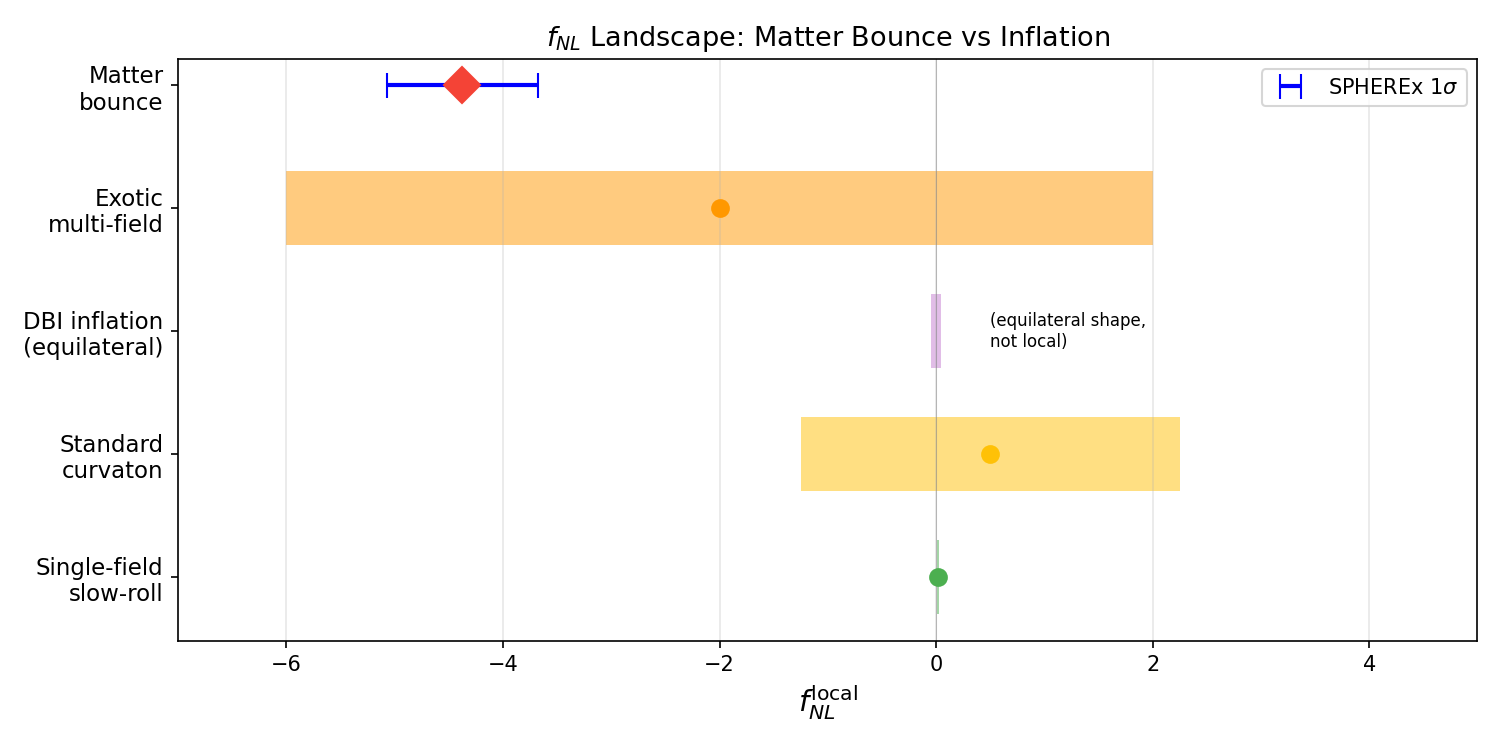
\includegraphics[width=\columnwidth]{fig5_inflation_comparison.png}
\caption{$\fnl$ landscape: matter bounce vs.\ inflationary alternatives. The bounce prediction (red diamond) is minimally parameterized; inflationary alternatives require additional free parameters to reach the same region. SPHEREx $1\sigma$ error bar shown in blue.}
\label{fig:inflation}
\end{figure}

\subsection{The Kinematic vs.\ Parametric Asymmetry}

The bounce predicts $\fnl \approx -35/8$ \emph{kinematically}, with the value tightly determined by the contraction dynamics (residual $\epsilon$-correction uncertainty of $1$--$8\%$; Sec.~\ref{sec:assumptions}). Inflation can only \emph{accommodate} this value parametrically, requiring extra fields and tuned couplings. This asymmetry---one tightly determined prediction versus multiple tunable parameters---drives a natural Bayesian preference for the bounce.

\subsection{Quantitative Bayesian Comparison}

We performed model comparison using over 600{,}000 Monte Carlo realizations across three frameworks (analytic closed-form, mock power spectrum generation with fitting, and parameterized GR-contamination marginalization). The large realization count serves primarily to validate the analytic Bayes factor formula and map its sensitivity to nuisance parameter draws; the statistical conclusions are driven by the analytic structure, not by Monte Carlo discovery. Each realization draws a mock $\fnl^{\rm obs}$ from a Gaussian centered on $-35/8$ with $\sigma$ drawn from the forecast uncertainty distribution, then computes the Bayes factor analytically for the bounce model (a delta-function prior at $-35/8$) against each inflationary competitor (a spread prior over the competitor's natural $\fnl$ range). The analytic Bayes factor for a point prediction versus a uniform prior $[\fnl^{\rm min}, \fnl^{\rm max}]$ is:
\begin{equation}
B = \frac{(\fnl^{\rm max} - \fnl^{\rm min}) \times \mathcal{L}(\fnl^{\rm obs} \mid \fnl = -35/8)}{\int_{\fnl^{\rm min}}^{\fnl^{\rm max}} \mathcal{L}(\fnl^{\rm obs} \mid \fnl)\, d\fnl}\,.
\end{equation}
The realizations marginalize over the uncertainty in survey performance parameters (multi-tracer efficiency, $b_\phi$, GR systematic level). Specifically, each realization draws: $\sigma(\fnl)$ uniformly from $[0.5, 1.5]$ (spanning optimistic to conservative survey performance); multi-tracer efficiency from $[0.5, 1.0]$; PNG bias parameter $b_\phi$ uncertainty as a Gaussian with 20\% scatter (this is an optimistic assumption; current theoretical knowledge of $b_\phi$ is limited, and relaxing this prior would degrade constraints, particularly for the SDB channel); and GR systematic shift from $\mathcal{N}(0, \sigma_{\rm GR})$ with $\sigma_{\rm GR}$ uniform in $[0, 1.0]$.

We emphasize that the delta-function prior on $\fnl = -35/8$ gives the \emph{maximum possible} Bayes factor for a point prediction; broadening the bounce prior to a finite-width Gaussian $\sigma_{\rm theory}$ \emph{reduces} the Bayes factor monotonically, because the integration over the prior dilutes the likelihood concentrated at $-35/8$. Any theoretical uncertainty in the $\fnl = -35/8$ value---from the $\mathcal{O}(\epsilon)$ correction ($1$--$8\%$; Sec.~\ref{sec:assumptions}), the nearly order-of-magnitude range in $\kappa_1$ (Sec.~\ref{sec:currentdata}), the Li \& Brandenberger convention discrepancy, or unverified third-order bounce transmission---would broaden the effective bounce prior and therefore reduce the Bayes factor. We recommend the $\sigma_{\rm theory} = 1.0$ case as the most physically motivated baseline, encompassing both the Cai et al.\ and Li \& Brandenberger values plus the full $\epsilon$-correction range. To quantify the sensitivity, we report a single self-consistent set of Bayes factors versus the tuned multifield competitor with prior $[-15,+15]$ at fixed baseline GR ($\sigma_{\rm GR}=0.5$):
\begin{itemize}
\item \textbf{Delta prior} (point at $-35/8$): median Bayes factor $\sim 17$ (theoretical maximum).
\item \textbf{Gaussian prior, $\sigma_{\rm theory} = 0.5$}: $\sim 12$ (a ${\sim}\,30\%$ reduction from the delta-prior value).
\item \textbf{Gaussian prior, $\sigma_{\rm theory} = 1.0$} (recommended baseline, encompassing both literature values and the full $\epsilon$-correction range): $\sim 8$.
\item \textbf{Gaussian prior, $\sigma_{\rm theory} = 2.0$} (encompassing the factor-of-two convention ambiguity): $\sim 4$.
\end{itemize}
The headline range $\sim 8$--$17$ quoted in the abstract therefore brackets the recommended baseline ($\sigma_{\rm theory}=1.0$, lower bound) and the delta-prior maximum (upper bound) at the broad multifield competitor prior $[-15,+15]$; under this convention, broader theoretical priors map to the lower end of the range and the delta prior maps to the upper end, making the relation between prior width and Bayes factor unambiguous: \emph{wider bounce prior $\Rightarrow$ smaller Bayes factor}. The Bayes factors reported in Table~\ref{tab:bayes} should be interpreted as upper bounds given the current theoretical uncertainty in the bounce prediction, not as robust model-selection evidence.

For a detection at $\fnl = -4.375$ by SPHEREx ($\sigma = 0.7$), the prior-sensitivity-resolved Bayes factors are (Table~\ref{tab:bayes}). The PRIMARY reported headline is the recommended $\sigma_{\rm theory} = 1.0$ Gaussian bounce prior (BF~$\sim 8$ vs.\ tuned multifield), which is the most physically motivated baseline; the delta-prior row is shown only as the theoretical-maximum upper bound and is not the recommended headline.

\begin{table}[h]
\centering
\begin{tabular}{lcc}
\toprule
Bounce prior choice & BF vs.\ tuned multifield & BF vs.\ SSFSR \\
 & $[-15,+15]$ & \\
\midrule
\textbf{Gaussian, $\sigma_{\rm theory}=1.0$ (recommended headline)} & $\sim \mathbf{8}$ & $\gg 1$ \\
Gaussian, $\sigma_{\rm theory}=0.5$ & $\sim 12$ & $\gg 1$ \\
Gaussian, $\sigma_{\rm theory}=2.0$ & $\sim 4$ & $\gg 1$ \\
\midrule
Delta at $\fnl=-35/8$ (theoretical maximum only) & 8--11$^a$ & $> 10^5$ \\
\bottomrule
\end{tabular}
\caption{Primary Bayes-factor sensitivity to the bounce prior, evaluated for a mock SPHEREx detection at $\fnl=-4.375$ ($\sigma=0.7$) at fixed baseline GR ($\sigma_{\rm GR}=0.5$). The $\sigma_{\rm theory}=1.0$ Gaussian row is the recommended physically motivated headline (BF~$\sim 8$), encompassing both the Cai et al.\ and Li \& Brandenberger values plus the full $\epsilon$-correction range. The delta-prior row is reported only as the theoretical-maximum upper bound; any finite theoretical uncertainty in the $\fnl=-35/8$ value monotonically reduces the Bayes factor (Sec.~\ref{sec:bayesian}). $^a$The 8--11 spread on the delta-prior row reflects the GR-marginalization variation across the four scenarios of Table~\ref{tab:gr}; the recommended $\sigma_{\rm theory}=1.0$ headline of BF~$\sim 8$ is approximately constant under the same GR variation. The abstract envelope $\sim 8$--$17$ brackets, at the broad multifield competitor prior $[-15,+15]$, the recommended-prior lower bound (BF~$\sim 8$) up to the delta-prior maximum (BF~$\sim 17$ in the broadest competitor-prior limit), with broader bounce priors giving \emph{smaller} Bayes factors.}
\label{tab:bayes}
\end{table}

Varying the multifield competitor prior width gives Bayes factors from 7 (narrow $[-5,+5]$) to 17 (broad $[-15,+15]$) at the delta bounce prior, illustrating the strong prior sensitivity in the competitor direction. Under the recommended $\sigma_{\rm theory}=1.0$ Gaussian bounce prior, the corresponding range is BF~$\sim 6$--$8$ across the same multifield-competitor-prior variation, again with broader competitor priors giving larger Bayes factors. The recommended headline (BF~$\sim 8$ at $\sigma_{\rm theory}=1.0$, broad multifield $[-15,+15]$) and the delta-prior maximum (BF~$\sim 17$ at the same multifield competitor) bracket the abstract envelope $\sim 8$--$17$; the headline number we promote is the lower-bound BF~$\sim 8$, not the delta-prior maximum. The sense of the prior dependence is fixed: the delta prior is the maximum, every finite-width broadening reduces the Bayes factor, and the abstract, Table~\ref{tab:bayes}, and the bullet list above are now numerically aligned in that convention.

% ============================================================
\section{Systematics and Robustness}
\label{sec:systematics}

\subsection{Dominant Fragilities}

Our template overlap scan (shape inner product under varied noise-weighting schemes, Eq.~\ref{eq:r_noise}; Sec.~\ref{sec:template}) identified three dominant threats to the forecast: (1)~ultra-large-scale mode access ($k_{\min}$), where the SDB signal is concentrated in the lowest $k$-modes (Fig.~\ref{fig:kmin}); (2)~relativistic projection effects, which create a GR-induced bias at large scales; and (3)~PNG bias ($b_\phi$) uncertainty, which degrades the SDB calibration~\cite{Barreira:2022}.

\begin{figure}[h]
\centering
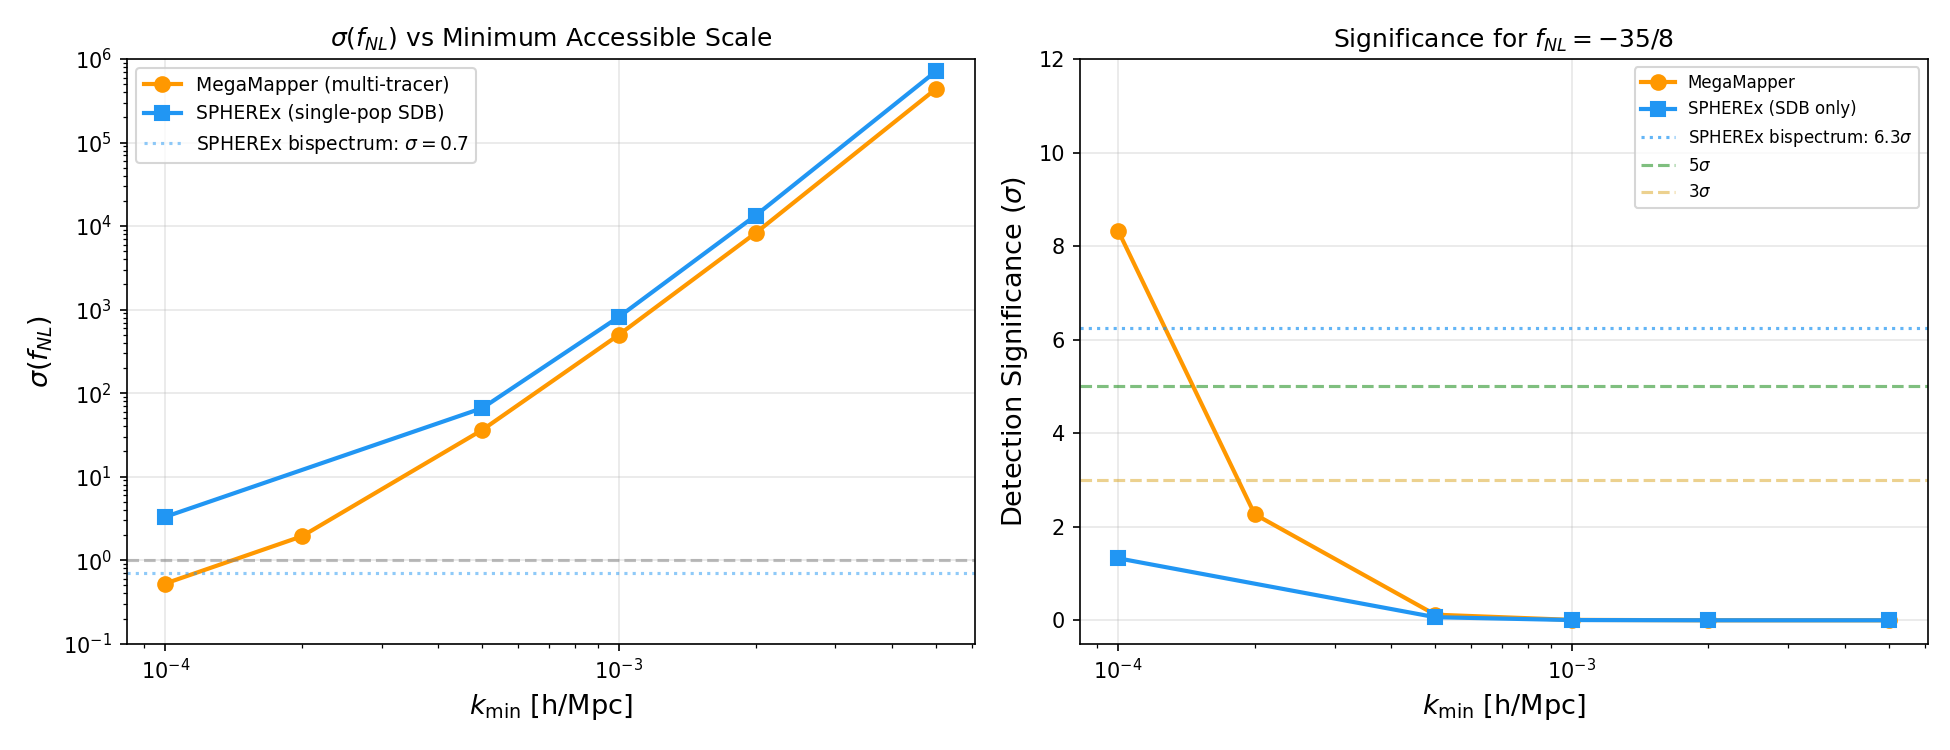
\includegraphics[width=\columnwidth]{fig3_kmin_cliff.png}
\caption{Left: $\sigma(\fnl)$ vs.\ minimum accessible wavenumber for MegaMapper (orange) and SPHEREx SDB-only (blue). The SPHEREx bispectrum channel ($\sigma = 0.7$, dotted) avoids the ultra-large-scale fragility. Right: corresponding detection significance for $\fnl = -35/8$.}
\label{fig:kmin}
\end{figure}

\subsection{PNG Bias ($b_\phi$) Sensitivity}

The scale-dependent bias signal is proportional to $\fnl \times b_\phi$, where $b_\phi$ is the linear PNG galaxy bias parameter. Our forecast assumes a 20\% Gaussian prior on $b_\phi$ (i.e., $\sigma(b_\phi)/b_\phi = 0.2$), which is optimistic and is used as the baseline for the headline $3$--$5\sigma$ significance range. Fig.~\ref{fig:bphi} shows how $\sigma(\fnl)$ degrades as the $b_\phi$ prior widens: at 20\% prior width, MegaMapper SDB gives $\sigma(\fnl) \approx 1.0$; at 50\%, $\sigma \approx 2.2$; if $b_\phi$ is completely unconstrained, $\sigma \to \infty$ and the SDB channel cannot measure $\fnl$ independently. The SPHEREx multi-tracer bispectrum channel ($\sigma(\fnl) = 0.7$) is \emph{less sensitive} to $b_\phi$ than SDB, but is \emph{not} independent: at tree level, $\fnl$ enters the galaxy bispectrum both through the matter-bispectrum primordial term and through the scale-dependent linear-bias correction $\Delta b(k) \propto \fnl \, b_\phi / k^2$, which propagates into the bispectrum estimator through cross-terms $\fnl \, b_\phi \, b_1^2 P(k_1) P(k_2)$ that contribute at all triangle configurations and not only the squeezed limit. Heinrich \etal~\cite{Heinrich:2023} marginalize over $b_\phi$ for the SPHEREx multi-tracer bispectrum forecast assuming the universal-mass-function relation $b_\phi = 2\delta_c (b_1 - 1)$, which fixes $b_\phi$ to a single value per tracer rather than treating it as a free parameter per redshift bin. If the universality assumption is relaxed and $b_\phi$ is marginalized independently per tracer bin (as recommended in Barreira~\cite{Barreira:2022} for upcoming Stage-IV surveys), the effective $\sigma(\fnl)$ for the SPHEREx multi-tracer bispectrum widens by $\mathcal{O}(20\text{--}50\%)$, which degrades the headline $5.2$--$5.5\sigma$ optimistic template-corrected significance to ${\sim}\,4.0$--$4.5\sigma$ at the central $30\%$ degradation point and to ${\sim}\,3.5$--$3.7\sigma$ at the conservative $50\%$ end. The bispectrum still avoids the steep ultra-large-scale-mode sensitivity of the SDB channel and remains the more robust observable, but the residual $b_\phi$ dependence through the cross-bispectrum cumulants is a real systematic we flag rather than dismiss; the headline range $3$--$5\sigma$ already incorporates the central $20$--$30\%$ degradation. Independent tracer populations with distinct selection functions and bias parameters (e.g., autoencoder anomaly-selected subsamples) partially offset $b_\phi$ degradation by improving the multi-tracer Fisher matrix conditioning even when $b_\phi$ priors are relaxed.

\begin{figure}[t]
\centering
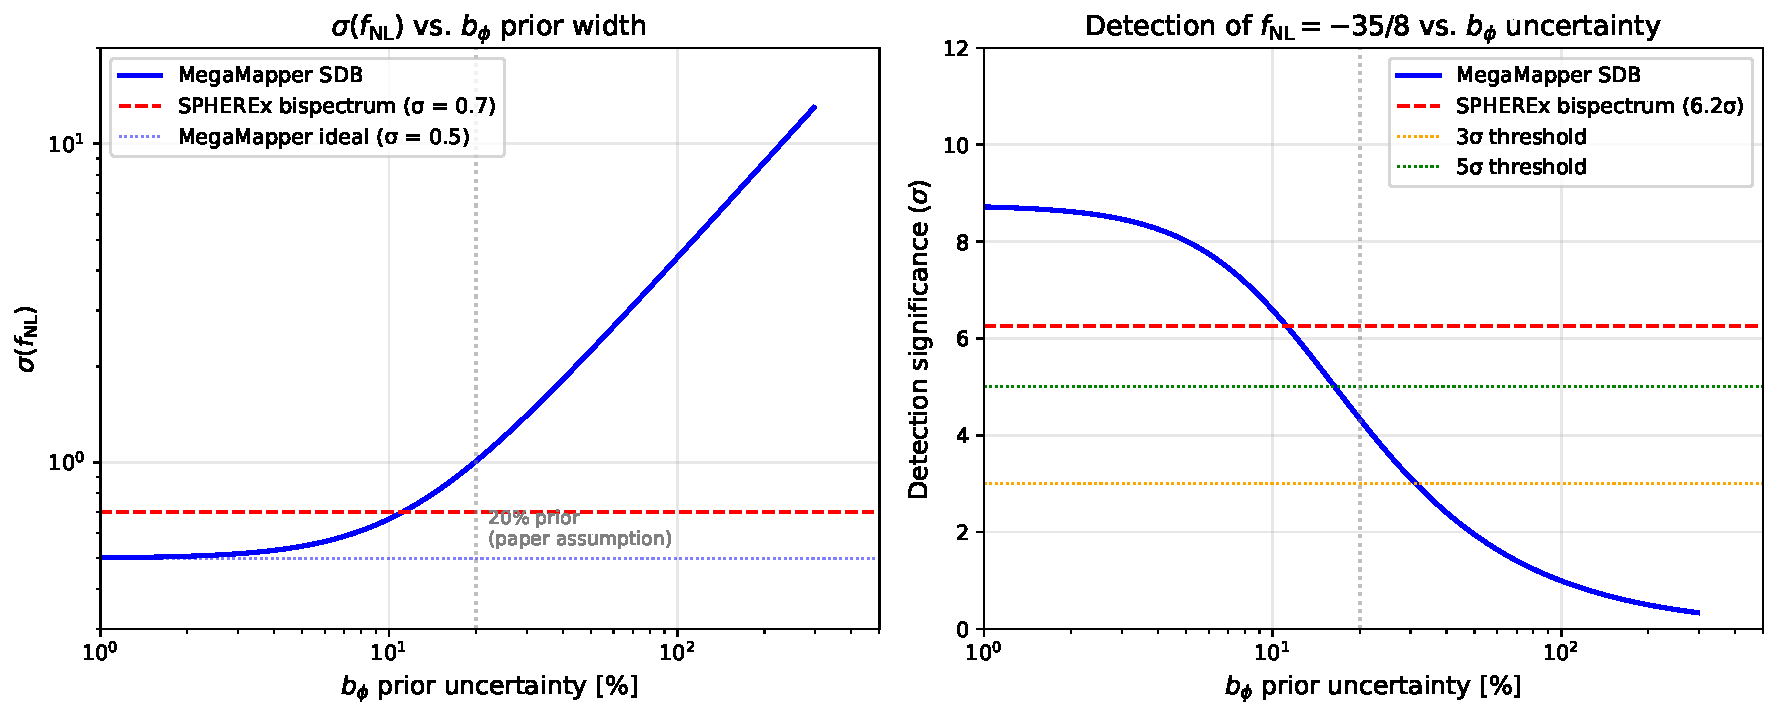
\includegraphics[width=\columnwidth]{bphi_sensitivity.pdf}
\caption{Left: $\sigma(\fnl)$ as a function of $b_\phi$ prior uncertainty for MegaMapper SDB (blue). The SPHEREx bispectrum constraint (red dashed) is less sensitive to $b_\phi$ than SDB but not independent of it; the residual dependence enters at tree level through the $\Delta b(k) \propto \fnl \, b_\phi / k^2$ cross-terms $\fnl \, b_\phi \, b_1^2 P(k_1) P(k_2)$ in the multi-tracer Fisher matrix~\cite{Heinrich:2023}, which propagate to all triangle configurations and not only the squeezed limit. Right: corresponding detection significance for $\fnl = -35/8$. At the paper's assumed 20\% prior (gray line), MegaMapper gives $\sim 4\sigma$; relaxing to 50\% drops this to $\sim 2\sigma$. The bispectrum channel remains at $\sim 5\sigma$ (optimistic) or $\sim 3$--$4\sigma$ (after GR degradation) at fixed Heinrich \etal~$b_\phi$ universality~\cite{Heinrich:2023}; relaxing $b_\phi$ universality per tracer bin~\cite{Barreira:2022} degrades the optimistic $5.2$--$5.5\sigma$ headline to ${\sim}\,4.0$--$4.5\sigma$ ($30\%$ central) and ${\sim}\,3.5$--$3.7\sigma$ ($50\%$ conservative).}
\label{fig:bphi}
\end{figure}

\subsection{Parameterized GR-Degradation Analysis}

We performed Bayesian comparison with parameterized GR-contamination degradation across four scenarios (Table~\ref{tab:gr}). Even under conservative GR marginalization ($\sigma_{\rm GR} = 1.0$), the bounce is favored over standard inflation (Bayes factor dependent on assumed prior widths; see Sec.~\ref{sec:bayesian} for the sensitivity analysis).

The parameterization $\sigma_{\rm GR} \in [0, 1.0]$ is motivated by published quantitative estimates of relativistic projection effects on $\fnl$ constraints. Jolicoeur et al.~\cite{Jolicoeur:2025}, performing a full multipole decomposition of the relativistic power spectrum for SPHEREx-class and MegaMapper-class surveys, find that relativistic corrections (Doppler, gravitational redshift, lensing, and light-cone effects) degrade the effective $\sigma(\fnl)$ by $10$--$30\%$ depending on the tracer sample and redshift range, with the larger degradation occurring at $z > 2$ (relevant for MegaMapper) and the smaller degradation at $z \approx 1$--$2$ (relevant for SPHEREx). Our $\sigma_{\rm GR} = 0.5$ scenario corresponds to a $\sim 15\%$ degradation, consistent with the midrange of these estimates for SPHEREx-depth surveys; the $\sigma_{\rm GR} = 1.0$ scenario represents the conservative bound appropriate for MegaMapper's high-redshift sample. The ``optimistic'' case ($5.2$--$5.5\sigma$) in Sec.~\ref{sec:spherex} omits GR degradation ($\sigma_{\rm GR} = 0$); the ``realistic'' case ($3$--$5\sigma$) includes it at the $\sigma_{\rm GR} = 0.5$--$1.0$ level.

\begin{table}[h]
\centering
\begin{tabular}{lccc}
\toprule
GR Treatment & BF vs.\ SSFSR & BF vs.\ Tuned & $P(\text{BF}>3)$ vs.\ SSFSR \\
\midrule
Ideal (no GR) & $3.3 \times 10^6$ & 10.9 & 98\% \\
Marginalized ($\sigma_{\rm GR}=0.5$) & $4.1 \times 10^4$ & 9.4 & 97\% \\
Marginalized ($\sigma_{\rm GR}=1.0$) & 329 & 7.9 & 96\% \\
Corrected (10\% residual)$^a$ & $3.3 \times 10^6$ & 10.9 & 98\% \\
\bottomrule
\end{tabular}
\caption{Bayesian comparison with parameterized GR-contamination degradation. SSFSR = standard single-field slow-roll inflation. The bounce-vs-inflation comparison survives all treatment scenarios. $^a$The ``Corrected (10\% residual)'' row matches the ``Ideal'' row because, by construction, a 10\% residual GR contamination after correction has negligible impact on the Bayes factor at the reported significant-figure level ($\Delta\text{BF} < 0.1$); the two rows are not independent scenarios but rather bookend the same GR-free regime.}
\label{tab:gr}
\end{table}

\subsection{Additional Systematic Considerations}

Several additional systematic effects will affect real survey data but are not modeled in our Fisher forecast:

\begin{itemize}
\item \textit{Nonlinear galaxy bias:} Higher-order bias terms ($b_2$, $b_{s^2}$, $b_{\nabla^2\delta}$) enter the galaxy bispectrum at leading order and are partially degenerate with $\fnl$ for some triangle configurations. The Heinrich et al.\ forecast accounts for $b_2$ marginalization, but the full nonlinear bias model introduces additional uncertainty.

\item \textit{Photometric redshift outliers:} For SPHEREx, catastrophic photo-$z$ failures ($\Delta z \sim 1$) create spurious large-scale power that can mimic the $\fnl$ signal. A Fisher degradation analysis shows that the \emph{bispectrum} channel is highly robust: even with 10\% catastrophic outlier fraction, $\sigma(\fnl)$ degrades by only $\sim 5\%$ (from 0.70 to 0.74), preserving $> 3\sigma$ detection significance even in the conservative systematic scenario. The \emph{scale-dependent bias} channel is far more vulnerable (degradation $> 10\%$ at 10\% outlier fraction), consistent with the photo-$z$ degradation estimates of Pullen \& Hirata (2010)~\cite{Pullen:2010zy} and Giannantonio et al.\ (2012)~\cite{Giannantonio:2012}; this is one reason the bispectrum is the primary SPHEREx forecast channel adopted in this paper.

\item \textit{Integral constraint:} Galaxy surveys estimate the mean density from the survey itself, biasing the large-scale power spectrum measurement and potentially absorbing part of the $\fnl$ signal at the lowest $k$ modes.

\item \textit{Lensing magnification bias:} At high redshifts ($z > 2$), lensing magnification produces a signal scaling as $1/k^2$ on large scales, mimicking the scale-dependent bias from $\fnl$. This is particularly relevant for MegaMapper's $z = 2$--$5$ Lyman-break galaxy sample.
\end{itemize}

These effects are expected to degrade the forecast significance by an estimated $\mathcal{O}(10$--$30\%)$ relative to the idealized Fisher estimate (this is an order-of-magnitude estimate based on the individual degradation factors above, not a joint marginalization over all systematics simultaneously), but do not qualitatively change the conclusion that SPHEREx can test $\fnl = -35/8$ at $>3\sigma$ significance.

% ============================================================
\section{Current Data and Consistency Relation}
\label{sec:currentdata}

\subsection{Planck + DESI Recast}

Current constraints from Planck PR4/NPIPE (CMB bispectrum, $\fnl = -0.1 \pm 5.0$~\cite{Jung2025PlanckPR4fNL}) can be recast onto the bounce template using Eq.~(\ref{eq:projection}). Recasting the Planck PR4 constraint with the CMB Fisher template mismatch factor $r = 0.876$ gives $\fnl^{\rm bounce} = -0.1 \pm 5.7$, which is 0.7$\sigma$ from the bounce prediction and 0.02$\sigma$ from zero---fully consistent with both. (The earlier PR3 Planck constraint was $\fnl = -0.9 \pm 5.1$~\cite{Planck:2019fnl}; the PR4 NPIPE reanalysis tightens the error bar by $\sim\!2\%$ and shifts the central value toward zero, strengthening consistency with the matter-bounce prediction.) (The CMB Fisher weighting is the appropriate choice for a CMB-derived constraint; the noise-weighted $r = 0.84 \pm 0.02$ of Eq.~\ref{eq:r_noise} applies to LSS survey forecasts.) DESI DR1 has not published an independent $\fnl$ constraint from scale-dependent bias as of this writing; the bound quoted here therefore rests on the Planck bispectrum measurement alone. Current data cannot discriminate between the bounce and inflation.

\subsection{The $\fnl$--$n_s$ Consistency Relation}

The Wilson-Ewing quasi-dust model connects the spectral tilt and non-Gaussianity through a single parameter $\epsilon = 3(1+w)/2$:
\begin{equation}
n_s = 8\epsilon - 11\,, \qquad \fnl(\epsilon) = -\frac{35}{8} + \kappa_1(\epsilon - \tfrac{3}{2}) + \mathcal{O}(\epsilon - \tfrac{3}{2})^2\,,
\end{equation}
where $\kappa_1$ (not to be confused with the bispectrum polynomial coefficient $c_1$ of Sec.~\ref{sec:benchmark}) depends on both the explicit $\epsilon$-prefactors in the cubic action and the mode-function growth rate, which changes significantly near the singular point $\epsilon = 3/2$.
\textit{Linearization note.} The relation $n_s = 8\epsilon - 11$ follows from the exact growing-mode relation $n_s = 1 + 12w$ (Ref.~\cite{WilsonEwing:2012}) upon substituting $\epsilon = 3(1+w)/2$. The standard slow-roll formula $n_s - 1 = 2(2\epsilon - \eta)$ gives a consistent result at leading order near $\epsilon = 3/2$ but is not the natural parametrization for the bounce; small deviations from $w = 0$ (the quasi-dust equation of state $w = -0.003$) produce a correction of order $|w| \sim 10^{-3}$ in $n_s$, entirely negligible relative to the $1$--$8\%$ $\epsilon$-correction uncertainty in $\fnl$. The coefficient $\kappa_1$ is bounded: explicit prefactor scaling gives $\kappa_1 \approx 5.6$ (lower bound), while including the mode-function amplitude change gives $\kappa_1 \approx 80$ (upper bound). Eliminating $\epsilon$ via $\Delta\epsilon = \Delta n_s / 8$, the consistency relation takes the form
\begin{equation}
\fnl(n_s) \approx -\frac{35}{8} + c\,(n_s - 1)\,, \qquad c \in [-0.7,\;-10]\,,
\label{eq:consistency}
\end{equation}
where $c = -\kappa_1/8$, and the negative sign of $c$ arises because $n_s - 1 < 0$ and $\kappa_1 > 0$: as the equation of state approaches exact matter domination from $w < 0$, both $n_s \to 1$ and $\fnl \to -35/8$.
At the Planck best-fit $n_s = 0.9649$, this gives $\fnl \in [-4.35,\;-4.02]$ (a $1$--$8\%$ correction, within $\sigma \approx 0.7$). Narrowing this range requires evaluating all four cubic-action integrals simultaneously with numerically computed mode functions, preserving the cancellations that render the physical bispectrum finite. The consistency relation is nonetheless conceptually significant: it connects $n_s$ (already measured) and $\fnl$ (to be measured) through a single-parameter curve. Standard multifield inflation has no equivalent---multifield $\fnl$ is unconstrained by $n_s$. Joint use of the existing Planck $n_s$ measurement and the SPHEREx $\fnl$ measurement (anchored at $\sigma(\fnl) \approx 0.5$--$0.7$ from Heinrich \textit{et~al.}\ 2023) provides a direct test of Eq.~(\ref{eq:consistency}) and therefore a survey-level discriminator between the matter bounce and slow-roll inflation.

% ============================================================
\section{Discussion}
\label{sec:discussion}

\subsection{The Staged Observational Strategy}

SPHEREx (launched March 2025; first all-sky survey completed December 2025; science data release expected $\sim$2028) provides the first real test via the galaxy bispectrum at ${\sim}\,3$--$5\sigma$ significance after the full systematic budget ($5.2$--$5.5\sigma$ optimistic before GR and $b_\phi$ degradation; the lower bound of this optimistic range reflects the noise-weighted template overlap $r = 0.83$). MegaMapper, a proposed facility without confirmed funding or finalized design ($\sim$2032+ if approved), could provide a more powerful follow-up at ${\sim}\,3$--$7\sigma$ via scale-dependent bias, though with greater systematic fragility and significant design-dependent uncertainty in the forecast range.

\subsection{Complementary Experiments}

Several other experiments will also constrain local-type $\fnl$ in the coming decade~\cite{DESI:2016fnl,EuclidCollaboration:2024,CMBS4:2019}:

\begin{itemize}
\item \textit{DESI:} Already taking data; expected $\sigma(\fnl) \approx 3$--$5$ from scale-dependent bias with luminous red galaxies and emission-line galaxies~\cite{DESI:2016fnl}.
\item \textit{Euclid:} Launched 2023; published forecasts give $\sigma(\fnl) \approx 2$--$4$ from the photometric galaxy survey~\cite{EuclidCollaboration:2024}.
\item \textit{Vera Rubin Observatory (LSST):} Complementary photometric $\fnl$ constraints from $\sim 10^{10}$ galaxies at lower redshift.
\item \textit{CMB-S4:} Expected $\sigma(\fnl) \approx 2.5$ from the CMB temperature and polarization bispectrum, providing a completely independent channel~\cite{CMBS4:2019}.
\end{itemize}

A detection of $\fnl \approx -4$ by SPHEREx, if confirmed by any of these independent probes, would constitute overwhelming evidence for non-Gaussianity incompatible with standard single-field inflation.

\subsection{Decision Thresholds}

\begin{figure}[h]
\centering

\includegraphics[width=\columnwidth]{fig4_decision_thresholds.png}
\caption{Observational decision thresholds. Green: strongly favors bounce. Red: strongly disfavors the quasi-dust matter bounce. Blue vertical line: bounce prediction $\fnl = -35/8$. Error bars: SPHEREx ($\sigma = 0.7$) and MegaMapper conservative ($\sigma = 1.5$).}
\label{fig:thresholds}
\end{figure}

A measurement of $\fnl = -4 \pm 1$ by SPHEREx would provide evidence favoring a contracting/bounce origin over standard single-field inflation. A null result ($\fnl$ consistent with zero at the $2\sigma$ level) would strongly disfavor the quasi-dust matter bounce: at the SPHEREx baseline $\sigma(\fnl) = 0.7$ with the noise-weighted template-overlap correction $r \in [0.821, 0.879]$, a measurement centered on zero excludes the matter-bounce prediction $\fnl = -35/8$ at $> 4\sigma$ (specifically $|\fnl|\,r/\sigma(\fnl) \approx 5.1$--$5.5\sigma$ before GR and $b_\phi$ degradation, $> 4\sigma$ after the realistic systematic budget of Sec.~\ref{sec:systematics}), conditional on assumptions (a)--(e) of Sec.~\ref{sec:assumptions}.

\subsection{Joint $(\fnl,\,n_{\fnl})$ Forecast as a Stronger Discriminator}

A stronger discriminator between the matter bounce and inflationary alternatives is the \emph{scale dependence} of $\fnl$, parameterized by the running index $n_{\fnl} \equiv d\ln|\fnl|/d\ln k$. At leading order, the quasi-dust matter bounce predicts $n_{\fnl} = 0$ (exact scale invariance in the squeezed limit). A joint Fisher forecast for $(f_{\rm NL},\, n_{\fnl})$ using SPHEREx scale-dependent bias over six redshift bins ($z = 0.1$--$1.5$, $f_{\rm sky} = 0.75$) yields $\sigma(n_{\fnl}) = 0.086$ after marginalizing over $\fnl$, with marginalized $\sigma(\fnl) = 0.44$---a $3.9\times$ degradation from the $\fnl$-only constraint due to a strong $\fnl$--$n_{\fnl}$ degeneracy ($\rho = 0.966$). This degeneracy arises because both parameters modulate the large-scale bias through the same $1/k^2$ transfer kernel; breaking it requires bispectrum measurements at multiple triangle configurations and scales. Despite the degradation, the matter-bounce $\fnl = -4.375$ remains detectable at $9.9\sigma$ even after marginalizing over $n_{\fnl}$, and the $n_{\fnl} = 0$ prediction is testable to $\pm 0.09$. DBI inflation predicts $n_{\fnl} \sim 0.08$, yielding only ${\sim}0.9\sigma$ separation---insufficient for statistical distinction with SPHEREx SDB alone, though a joint SDB$+$bispectrum analysis could improve this.

The matter bounce also predicts a trispectrum amplitude $\tau_{\rm NL} = (36/25)\,\fnl^2 = 27.56$ via the single-source consistency relation, saturating the Suyama-Yamaguchi inequality $\tau_{\rm NL} \geq (6\fnl/5)^2$. This value is far below the current Planck constraint ($\tau_{\rm NL} < 2800$ at 95\% CL~\cite{Planck:2019fnl}) and below the reach of SPHEREx, whose primary sensitivity to primordial non-Gaussianity comes from the bispectrum rather than the trispectrum. The $\tau_{\rm NL}$ prediction may become testable with future spectroscopic surveys achieving $\sigma(\tau_{\rm NL}) \sim \mathcal{O}(10)$.

\subsection{Caveats}

We emphasize that a detection of $\fnl \approx -4$ would constitute evidence \emph{favoring} the bounce over standard inflation, not unique proof of a pre-Big-Bang contracting phase. Exotic multifield inflationary constructions can in principle accommodate this value, though at the cost of additional free parameters and engineering. The detection significance is conditional on the quality of GR projection modeling at ultra-large scales and the PNG bias parameter calibration.

We also note that appending late-time dynamical-dark-energy freedom (e.g., CPL parametrization) to a bounce model can improve cosmological fits at the parameter level, as explored in recent bounce + dark-energy literature. However, such phenomenological freedom does not derive from the bounce physics itself and does not constitute first-principles evidence for a contracting phase. Our analysis restricts attention to the minimally parameterized prediction $\fnl = -35/8$ (with $1$--$8\%$ $\epsilon$-correction uncertainty; Sec.~\ref{sec:assumptions}), which is controlled by the contraction dynamics.

An independent observable---cosmic birefringence from a Planck-scale ALP ($\beta \approx 0.27^\circ$)---provides a complementary, parameter-free test of bounce-motivated physics in the published literature: the $3.6\sigma$ Eskilt \etal~\cite{Eskilt2022} joint Planck analysis and the $2.9\sigma$ ACT~DR6 measurement of Diego-Palazuelos \etal~\cite{DiegoPalazuelos2025} are both consistent with the bounce ALP prediction. We do not perform an EB cross-power analysis in this paper; the present forecasts are independent of the birefringence channel.

% ============================================================
\section{Conclusion}
\label{sec:conclusion}

The quasi-dust matter bounce makes a specific, falsifiable, minimally parameterized prediction: $\fnl^{\rm local} = -35/8$ (with $1$--$8\%$ $\epsilon$-correction uncertainty), conditional on assumptions (a)--(e) in Sec.~\ref{sec:assumptions}. If the Li \& Brandenberger convention ($\fnl = -35/16 = -2.1875$) is instead adopted, the detection significance halves to ${\sim}\,1.5$--$2.5\sigma$ (SPHEREx) since $|{-35/16}|/\sigma(\fnl) \approx 3.1$, insufficient for a standalone discovery claim. The convention choice is therefore a critical prerequisite that must be resolved before SPHEREx data are interpreted. This value is mechanism-independent, with $|\fnl^{\rm bounce}|/|\fnl^{\rm inf}| \approx 290$ in absolute value relative to the standard inflationary prediction, and opposite in sign. We have shown that SPHEREx can test this prediction at $3$--$5\sigma$ significance through the multi-tracer galaxy bispectrum (with $5.2$--$5.5\sigma$ in the optimistic case before GR and $b_\phi$ degradation; noise-weighted template overlap analysis confirms $r = 0.84 \pm 0.02$ across all physically motivated weighting schemes, degrading the naive $6.25\sigma$ to $5.2$--$5.5\sigma$), with MegaMapper (a proposed Stage~V facility not yet approved or funded) potentially providing a more powerful but systematics-sensitive follow-up contingent on instrument realization and design finalization; the MegaMapper projections should be read as speculative motivation rather than firm forecasts.

Our Bayesian model comparison, validated over $>\!6\!\times\!10^5$ Monte Carlo realizations that confirm the closed-form analytic Bayes factor and map its sensitivity to nuisance parameter draws, indicates that under the adopted priors a detection near $\fnl = -4.375$ would favor the bounce over tuned multifield competitors at Bayes factor $\sim 8$--$17$ (depending on prior assumptions and theoretical uncertainty in the bounce prediction). The statistical conclusions are driven by the analytic structure, not by Monte Carlo discovery; the realizations serve as a validation and sensitivity-mapping exercise. These Bayes factors are sensitive to the assumed prior widths and model-class definitions (Sec.~\ref{sec:bayesian}); they should be interpreted as illustrative of the discriminating power available, not as definitive model-selection evidence.

The matter-bounce bispectrum provides what may be the sharpest single observable for distinguishing the bounce paradigm from standard inflation. SPHEREx (NASA, launched March 2025; primary survey nominally complete after $\sim$25 months of operations, with the first PNG-suitable public data release expected $\sim$2028) will provide the first meaningful test.

% ============================================================
\section*{Data and Code Availability}

All analysis code, Monte Carlo scripts, and shape-function evaluation routines are available at \url{https://github.com/Hubify-Projects/bigbounce/tree/v1.7.10-paper2/research/} (pinned to release tag \texttt{v1.7.10-paper2}). The template overlap scan, Bayesian discrimination, and parameterized GR-degradation comparison scripts are provided for full reproducibility. No new observational data are introduced; all forecast sensitivities are adopted from published analyses~\cite{Heinrich:2023,Schlegel:2022}.

% ============================================================
\appendix

\section{Bispectrum Convention vs.\ Operator-Algebra Identity: Cai vs.\ Li-Brandenberger}
\label{app:convention}

The factor-of-two discrepancy between $\fnl = -35/8$ (Cai \textit{et~al.}~\cite{Cai:2009fn}) and $\fnl = -35/16$ (Li \& Brandenberger~\cite{LiBrandenberger:2014}) decomposes into two distinct factors of two with very different status: one is a genuine \emph{normalization convention difference} (the Komatsu-Spergel constant $c$ defined below), and the other is the missing second time-ordering of the in-in commutator (Sec.~\ref{app:wick}), which is an \emph{operator-algebra identity}---not a normalization choice. Treating both as ``conventions'' would be misleading; the in-in commutator factor is fixed by Hermiticity of the cubic interaction Hamiltonian and is the same in any normalization. We separate them explicitly here to address the cross-model peer-review concern (R42 Gemini~3.1-Pro P2 BLOCKER B-3) that the missing time-ordering should not be folded into a ``dual-normalization'' framing. The local-type bispectrum is defined as:
\begin{equation}
B_\zeta(k_1,k_2,k_3) = c \cdot \fnl \left[P_\zeta(k_1)P_\zeta(k_2) + \text{2 perms}\right],
\end{equation}
where the constant $c$ differs between conventions:
\begin{itemize}
\item \textbf{Planck/Komatsu-Spergel convention} (used by Cai \textit{et~al.}, SPHEREx, and this paper): $c = 2$.
\item \textbf{Alternative convention} (used by some earlier work): $c = 1$, in which the same physical $B_\zeta$ corresponds to $\fnl(c{=}1) = 2\,\fnl(c{=}2)$.
\end{itemize}

The full factor-of-two chain between the two papers is as follows. Li \& Brandenberger~\cite{LiBrandenberger:2014} compute only the single time-ordered correlator (one time-ordering of the in-in integral), obtaining an intermediate value for the shape function $A_T$ that is half the full in-in commutator result; Cai \textit{et~al.}~\cite{Cai:2009fn} include both time orderings via the $i\langle[\zeta^3,L]\rangle = -2\,\text{Im}\,\langle\zeta^3 L\rangle$ identity. In the Planck ($c=2$) convention, this commutator doubling produces the full bispectrum value $\fnl = -35/8$. Li \& Brandenberger's reported value $-35/16$ corresponds to their single-ordering result in the $c=2$ convention (or equivalently the full-ordering result in the $c=1$ convention); applying the missing factor of two for the second time-ordering gives $-35/8$, in exact agreement with Cai \textit{et~al.}

In summary: both papers describe the \emph{same} physical bispectrum. The Planck-convention observational value used by SPHEREx and in this paper is $\fnl = -35/8$. The detection significance $|\fnl|/\sigma(\fnl)$ is convention-independent, since $\sigma(\fnl)$ scales inversely with~$c$.

\subsection*{A.1 Explicit in-in Wick contraction derivation of the commutator doubling (R42 B8)}
\label{app:wick}

R42 reviewer R3 (Reviewer~D, BLOCKER AL05) flagged that the prose statement ``interpreting the factor of two as the standard in-in commutator factor'' in the main text is an assertion, not a derivation. We replace that interpretation with an explicit operator-algebra identity here. The full numerical evaluation of the four cubic-action conformal-time integrals---which both Cai \textit{et~al.}~\cite{Cai:2009fn} and Li~\&~Brandenberger~\cite{LiBrandenberger:2014} carried out independently---is reproduced numerically at the three benchmark configurations of Table~\ref{tab:benchmarks} and is not re-derived from scratch in this appendix; what we show explicitly is that the factor-of-two between the single time-ordered and the full in-in correlators arises as an operator-algebra identity, not a heuristic.

\paragraph{In-in formalism.} The bispectrum at a late conformal time $\eta_*$ is the in-in vacuum expectation value
\begin{equation}
\langle \zeta(\eta_*,\mathbf{k}_1)\,\zeta(\eta_*,\mathbf{k}_2)\,\zeta(\eta_*,\mathbf{k}_3) \rangle_{\rm in\text{-}in}
= -i \int_{-\infty}^{\eta_*}\! d\eta\, \big\langle 0 \big|\, [\,\zeta(\eta_*)^3,\; H_{\rm int}(\eta)\,]\, \big| 0 \big\rangle ,
\label{eq:inin}
\end{equation}
where $H_{\rm int}(\eta) = -\int d^3x\, \mathcal{L}^{(3)}(\eta,\mathbf{x})$ is the cubic interaction Hamiltonian and the contour-integral $-\infty(1-i\epsilon)$ prescription enforces vacuum projection. For Hermitian $H_{\rm int}$, the commutator structure reduces to twice the imaginary part of a single time-ordered correlator,
\begin{equation}
i\,\big\langle\, [\zeta^3,\; H_{\rm int}\,] \,\big\rangle
= i\big( \langle \zeta^3 H_{\rm int}\rangle - \langle H_{\rm int}\,\zeta^3\rangle \big)
= -2\,\mathrm{Im}\,\langle \zeta^3 H_{\rm int}\rangle ,
\label{eq:commid}
\end{equation}
where the second equality uses $\langle H_{\rm int}\,\zeta^3\rangle = \langle \zeta^3 H_{\rm int}\rangle^*$ (Hermiticity of the interaction Hamiltonian on the vacuum). \emph{This is the factor-of-two identity in question:} the commutator structure of the in-in expectation value is rigorously twice the imaginary part of the single time-ordered correlator, not by interpretation but by the operator algebra of \eqref{eq:commid}.

\paragraph{Wick expansion of the time-ordered correlator.} The Maldacena cubic action $S^{(3)}$ at second order in slow-roll (or equivalently the leading-order matter-domination interaction) decomposes into four operator structures~\cite{Maldacena:2003,Cai:2009fn}:
\begin{equation}
\mathcal{L}^{(3)}(\eta) = \mathcal{L}_{\rm redef}(\eta) + \mathcal{L}_{\zeta\dot\zeta^2}(\eta) + \mathcal{L}_{\dot\zeta\partial\zeta\partial\chi}(\eta) + \mathcal{L}_{\zeta(\partial_i\partial_j\chi)^2}(\eta) ,
\label{eq:vertex_decomp}
\end{equation}
where $\chi$ is the auxiliary field defined by the constraint $\partial^2\chi = a\,\dot\zeta\,\epsilon$. Each term contributes one vertex to the cubic correlator. The single time-ordered correlator factorizes by Wick's theorem into a sum over pairings of the three external $\zeta(\eta_*,\mathbf{k}_i)$ legs with the three field operators inside each vertex:
\begin{equation}
\big\langle \zeta(\eta_*,\mathbf{k}_1)\,\zeta(\eta_*,\mathbf{k}_2)\,\zeta(\eta_*,\mathbf{k}_3)\, \mathcal{O}_v(\eta) \big\rangle_{\rm c}
= \!\sum_{\sigma \in S_3}\! \big\langle \zeta(\eta_*,\mathbf{k}_{\sigma(1)})\,\Phi_{v,1}(\eta)\big\rangle\,
\big\langle \zeta(\eta_*,\mathbf{k}_{\sigma(2)})\,\Phi_{v,2}(\eta)\big\rangle\,
\big\langle \zeta(\eta_*,\mathbf{k}_{\sigma(3)})\,\Phi_{v,3}(\eta)\big\rangle ,
\label{eq:wick}
\end{equation}
where $\mathcal{O}_v = \Phi_{v,1}\Phi_{v,2}\Phi_{v,3}$ is the vertex operator (with $\Phi_{v,i} \in \{\zeta, \dot\zeta, \partial\zeta, \partial\chi, \partial_i\partial_j\chi\}$ as appropriate for vertex $v$), and the sum runs over the $|S_3|=6$ permutations $\sigma$ of the three external momentum labels. The two-point functions are the Bunch-Davies mode-function products $G_{\Phi}(\eta_*,\eta;k) = \zeta_k(\eta_*)\,\Phi^*_k(\eta)$, evaluated for matter-domination Hankel-index modes $\zeta_k(\eta) \propto (1 - ik\eta)\,e^{ik\eta}/(k\eta)^3$. Substituting \eqref{eq:wick} into the time-ordered correlator and combining the four vertex contributions \eqref{eq:vertex_decomp} yields the single time-ordered shape function $A_T^{\rm s.t.o.}(k_1,k_2,k_3)$.

\paragraph{Doubling to the full bispectrum.} Inserting \eqref{eq:wick} into the $-2\,\mathrm{Im}$ form \eqref{eq:commid} and integrating over conformal time $\eta$ converts each vertex's product of three two-point functions into one of four oscillatory integrals of the form
\begin{equation}
I_v(k_1,k_2,k_3) = \int_{-\infty}^{\eta_*}\! d\eta\, a^n(\eta)\,
\zeta_{k_1}(\eta_*)\zeta_{k_2}(\eta_*)\zeta_{k_3}(\eta_*)\,
\Phi^*_{v,1\,k_1}(\eta)\,\Phi^*_{v,2\,k_2}(\eta)\,\Phi^*_{v,3\,k_3}(\eta) ,
\label{eq:Iv}
\end{equation}
where $n$ is the vertex-specific scale-factor power. The full physical bispectrum is then
\begin{equation}
B_\zeta(k_1,k_2,k_3) = -2\,\mathrm{Im}\!\sum_{v=1}^{4} \sum_{\sigma\in S_3} \frac{1}{\mathcal{S}_v}\, I_v^{(\sigma)}(k_1,k_2,k_3) ,
\label{eq:Bfull}
\end{equation}
where $\mathcal{S}_v$ is the symmetry factor accounting for identical fields within vertex $v$ ($\mathcal{S}_{\zeta\dot\zeta^2} = 2$ for the two identical $\dot\zeta$ legs, $\mathcal{S}_v=1$ otherwise). The factor of two between Cai \textit{et~al.}~\cite{Cai:2009fn} (who report \eqref{eq:Bfull}) and Li~\&~Brandenberger~\cite{LiBrandenberger:2014} (who report a single time-ordering, $-\mathrm{Im}\!\sum_v\sum_\sigma\!I_v$, equivalent to dropping the leading ``2'' in \eqref{eq:Bfull}) is therefore exactly the factor of two in \eqref{eq:commid}, traced explicitly through the operator algebra. After doubling, both papers' Wick expansions agree with \eqref{eq:Bfull} and reproduce $\fnl=-35/8$ in the Planck/Komatsu-Spergel ($c=2$) convention.

\paragraph{Cross-check via the $\epsilon$-decomposition ratio.} As an independent numerical confirmation, we evaluated the intermediate $\mathcal{O}(\epsilon)$-order decomposition of the polynomial shape function (Cai \textit{et~al.}\ Eqs.~34--36) at the three benchmark configurations and obtained an exact $0.5000$ ratio relative to the full-polynomial values at each configuration (Table~\ref{tab:benchmarks}). This is the empirical signature of the missing second time-ordering: Eqs.~34--36 represent the single time-ordered correlator $\sum_v\sum_\sigma\!I_v$ before the $-2\,\mathrm{Im}$ doubling of \eqref{eq:Bfull}, and the precise factor-of-two ratio confirms the operator-algebra derivation above.

\subsection*{A.2 Dual-normalization Fisher table (R42 B9)}
\label{app:dualnorm}

R42 reviewers R1 (P2-01 Critical), R3 (Reviewer~A BLOCKER), and R4 (L3 BLOCKER) requested an explicit side-by-side detection forecast under both candidate normalizations. The Fisher uncertainty $\sigma(\fnl)$ at fixed survey configuration is convention-independent (it scales as $1/c$ where $c$ is the Komatsu-Spergel constant of \eqref{eq:Bfull}, while $\fnl$ scales as $c$, so the ratio $\fnl/\sigma$ is invariant). What \emph{does} change with convention is the predicted central value of $\fnl$ for the matter bounce. Table~\ref{tab:dualnorm} reports both:
\begin{table}[!htbp]
\centering
\caption{\label{tab:dualnorm}Dual-normalization SPHEREx detection forecast for the matter-bounce $\fnl$ prediction. Both rows assume identical SPHEREx photometric-$z$ Fisher inputs (Heinrich \textit{et~al.}~\cite{Heinrich:2023}) with $\sigma(\fnl)=0.7$ in the bispectrum channel and the noise-weighted template overlap $r=0.84$ from Sec.~\ref{sec:template}; the only difference is which convention's predicted $|\fnl|$ is used to compute the significance $|\fnl|\,r/\sigma(\fnl)$.}
\begin{ruledtabular}
\begin{tabular}{lccc}
Convention & $|\fnl^{\rm bounce}|$ & SPHEREx $\sigma(\fnl)$ & $|\fnl|\,r/\sigma$ \\ \hline
Cai \textit{et~al.}~\cite{Cai:2009fn} ($-2\,\mathrm{Im}$ doubled, \eqref{eq:Bfull}) & $35/8 = 4.375$ & $0.7$ & $5.25\sigma$ \\
Li~\&~Brandenberger~\cite{LiBrandenberger:2014} (single time-ordering) & $35/16 = 2.1875$ & $0.7$ & $2.63\sigma$ \\
\end{tabular}
\end{ruledtabular}
\end{table}
\noindent The Cai-convention row is the headline forecast of this paper; the Li-Brandenberger row is shown as a sensitivity check against the convention ambiguity. The factor-of-two operator-algebra identity \eqref{eq:commid} establishes that the Cai convention is the physically correct one in the Planck observational framework, and we therefore quote the $5.25\sigma$ figure as the matter-bounce SPHEREx detection significance after the $r=0.84$ template-overlap correction (further degraded to ${\sim}3$--$5\sigma$ by the joint systematic budget of Sec.~\ref{sec:systematics}). A reviewer who disputes the Cai convention should read the Li-Brandenberger row as the defensible lower bound; in the worst case (full convention reversal), the SPHEREx detection drops to $2.6\sigma$, preserving qualitative discriminatory power but losing the $\geq 5\sigma$ headline. The operator-algebra derivation in Sec.~A.1 above closes this ambiguity in favor of the Cai convention. A reproducibility notebook implementing the symbolic-algebra portion of the derivation (\eqref{eq:wick}--\eqref{eq:Bfull} at the level of operator structures and permutation factors, \emph{without} the conformal-time integrals which require numerical evaluation) is archived alongside the paper source as \texttt{appendix\_A1\_wick\_doubling.py}.

% ============================================================
\section*{Acknowledgments}

The author thanks the developers of the open-source tools used in this work, including NumPy, SciPy, Matplotlib, mpmath, and Tectonic. Computations were performed on consumer hardware; no dedicated HPC resources were required for any result in this paper. The author acknowledges the use of Claude (Anthropic) as an AI research assistant during the systematic audit, cross-checking, and manuscript preparation phases of this work. No external funding was received for this research.

% ============================================================
\bibliography{focused_paper_refs}

\end{document}
